\documentclass{article}
% generated by Madoko, version 1.0.0-rc5
%mdk-data-line={1}


\usepackage[heading-base={2},section-num={False},bib-label={True}]{madoko2}


\begin{document}



%mdk-data-line={7}
\mdxtitleblockstart{}
%mdk-data-line={7}
\mdxtitle{\mdline{7}Optimization of a DNN program on the CPU+MIC}%mdk
\mdxauthorstart{}
%mdk-data-line={12}
\mdxauthorname{\mdline{12}University of Electronic Secience and Technology of China}%mdk
\mdxauthorend\mdtitleauthorrunning{}{}\mdxtitleblockend%mdk

%mdk-data-line={9}
\begin{abstract}%mdk

%mdk-data-line={10}
\noindent\mdline{10}This article is a part of competition proposal of Asia Supercomputer Student Challenge. We analysis the \mdline{10}\mdcode{DNN}\mdline{10} program, put forward different optimization methods, test them and point their pros and cons. In the end we talk about our limits.%mdk
%mdk
\end{abstract}%mdk

%mdk-data-line={12}
\section{\mdline{12}1.\hspace*{0.5em}\mdline{12}Introduction}\label{sec-introduction}%mdk%mdk

%mdk-data-line={13}
\noindent\mdline{13}There is a program based on a standalone hybrid CPU+MIC platform called \mdline{13}\mdcode{DNN(deep~neural~network)}\mdline{13} needed to be parallelized for obtain better performance. Here is some detailed information about hardware in Figure 1, software configuration in Figure 2.%mdk

%mdk-data-line={15}
\mdline{15}After optimization, the final program is tested on one computing server in the CPU+MIC hybrid cluster. Performance analysis in this proposal is based on the results of this test.%mdk

%mdk-data-line={16}
\begin{figure}[tbp]%mdk
\begin{mdcenter}%mdk

%mdk-data-line={18}
\noindent\mdline{18}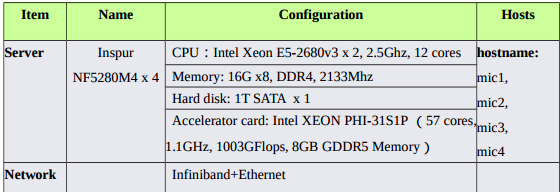
\includegraphics[keepaspectratio=true,width=\dimmin{}{\dimwidth{0.90}}]{images/2016-02-18-23-01-13-}{}\mdline{18}%mdk

%mdk-data-line={21}
\mdhr{}%mdk

%mdk-data-line={22}
\noindent\mdline{22}\mdcaption{\textbf{Figure~\mdcaptionlabel{1}.}~\mdcaptiontext{Hardware configuration}}%mdk
%mdk
\end{mdcenter}\label{fig-myfigure}%mdk
%mdk
\end{figure}%mdk

%mdk-data-line={23}
\begin{figure}[tbp]%mdk
\begin{mdcenter}%mdk

%mdk-data-line={24}
\noindent\mdline{24}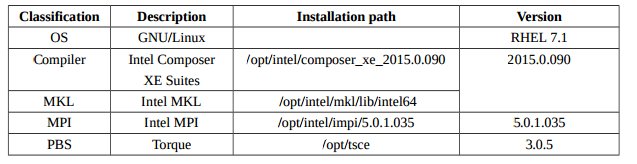
\includegraphics[keepaspectratio=true,width=\dimmin{}{\dimwidth{0.90}}]{images/2016-02-18-23-13-11-}{}\mdline{24}%mdk

%mdk-data-line={27}
\mdhr{}%mdk

%mdk-data-line={28}
\noindent\mdline{28}\mdcaption{\textbf{Figure~\mdcaptionlabel{2}.}~\mdcaptiontext{Software configuration}}%mdk
%mdk
\end{mdcenter}\label{fig-myfigure}%mdk
%mdk
\end{figure}%mdk

%mdk-data-line={29}
\section{\mdline{29}2.\hspace*{0.5em}\mdline{29}Analysis of the serial program}\label{sec-analysis-of-the-serial-program}%mdk%mdk

%mdk-data-line={30}
\subsection{\mdline{30}2.1.\hspace*{0.5em}\mdline{30}Coarse grain analysis}\label{sec-coarse-grain-analysis}%mdk%mdk

%mdk-data-line={31}
\noindent\mdline{31}At first, we generate a call graph(Figure 3) by using \mdline{31}\mdcode{Google~perfools}\mdline{31}, a open source performance profiler, to have a glance though it. Every square represents a function, and the bigger square is, the more time corresponding function cost.%mdk

%mdk-data-line={33}
\begin{figure}[tbp]%mdk
\begin{mdcenter}%mdk

%mdk-data-line={34}
\noindent\mdline{34}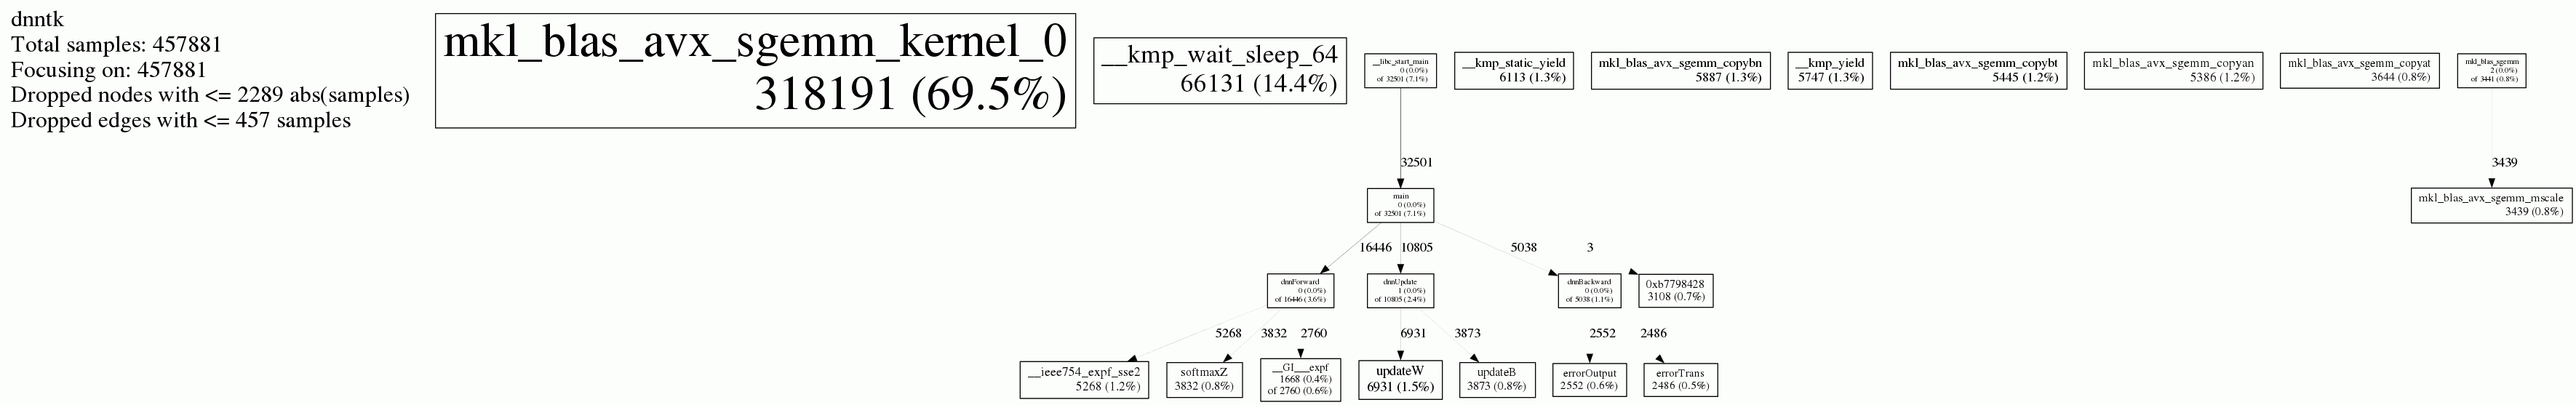
\includegraphics[keepaspectratio=true,width=\dimmin{}{\dimwidth{0.90}}]{images/100001994364201}{}\mdline{34}%mdk

%mdk-data-line={37}
\mdhr{}%mdk

%mdk-data-line={38}
\noindent\mdline{38}\mdcaption{\textbf{Figure~\mdcaptionlabel{3}.}~\mdcaptiontext{Google Perfools results}}%mdk
%mdk
\end{mdcenter}\label{fig-myfigure}%mdk
%mdk
\end{figure}%mdk

%mdk-data-line={38}
\mdline{38}Obviously, the hot spot is something about \mdline{38}\mdcode{MKL}\mdline{38}. After googling
and searching Intel document we know that MKL provides \mdline{39}\mdcode{BLAS~routinues}\mdline{39}, which includes a serial function named \mdline{39}\mdcode{cblas\_?gemm}\mdline{39}
to compute a matrix-matrix product with general matrices.%mdk

%mdk-data-line={42}
\mdline{42}But giving that MKL function is well-optimized, we search for all position where \mdline{42}\mdcode{cblas\_*gemm}\mdline{42} is called. Results show the usage of \mdline{42}\mdcode{cblas\_*gemm}\mdline{42} appear in file \mdline{42}\mdcode{dnn\_func.cpp}\mdline{42}, more specifically, in three functions:%mdk

%mdk-data-line={44}
\begin{itemize}[noitemsep,topsep=\mdcompacttopsep]%mdk

%mdk-data-line={44}
\item\mdline{44}\mdcode{\preindent{1}extern~"C"~int~dnnForward(NodeArg~\&nodeArg)}\mdline{44}%mdk

%mdk-data-line={45}
\item\mdline{45}\mdcode{\preindent{1}extern~"C"~int~dnnBackward(NodeArg~\&nodeArg)}\mdline{45}%mdk

%mdk-data-line={46}
\item\mdline{46}\mdcode{\preindent{1}extern~"C"~int~dnnUpdate(NodeArg~\&nodeArg)}\mdline{46}%mdk
%mdk
\end{itemize}%mdk

%mdk-data-line={48}
\noindent\mdline{48}They call \mdline{48}\mdcode{MKL}\mdline{48} function \mdline{48}\mdcode{cblas\_sgemm}\mdline{48} many times by \mdline{48}\mdcode{for~loop}\mdline{48} and 
cost almost 90\% of all CPU time. So we guess that those function
 is what we may optimize, aka, hotspots.
The report(see Figure 4.) showed by\mdline{51}\mdcode{Intel~VTune}\mdline{51}, another profiler, proves our guess.%mdk

%mdk-data-line={53}
\begin{figure}[tbp]%mdk
\begin{mdcenter}%mdk

%mdk-data-line={54}
\noindent\mdline{54}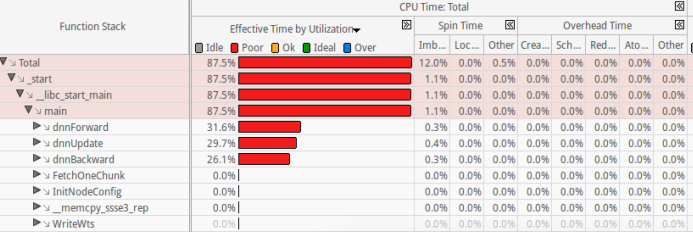
\includegraphics[keepaspectratio=true,width=\dimmin{}{\dimwidth{0.90}}]{images/2016-02-19-10-36-25-}{}\mdline{54}%mdk

%mdk-data-line={56}
\mdhr{}%mdk

%mdk-data-line={57}
\noindent\mdline{57}\mdcaption{\textbf{Figure~\mdcaptionlabel{4}.}~\mdcaptiontext{Intel VTune top-down tree}}%mdk
%mdk
\end{mdcenter}\label{fig-myfigure}%mdk
%mdk
\end{figure}%mdk

%mdk-data-line={58}
\mdline{58}According to a skim through the source code, we could establish a clear structure about this program. To simplify code, original program could be rewritten in pseudocode:%mdk
\begin{mdpre}%mdk
\noindent{\mdcolor{purple}1}.~{\mdcolor{teal}GetInitFileConfig}(cpuArg)\\
{\mdcolor{purple}2}.~{\mdcolor{teal}While}~{\mdcolor{teal}FetchOneChunk}(cpuArg,~onChunk)~{\mdcolor{navy}do}:\\
{\mdcolor{purple}3}.~~~~~~~{\mdcolor{teal}While}~{\mdcolor{teal}FetchOneBunch}(oneChunk,~nodeArg)~{\mdcolor{navy}do}:\\
{\mdcolor{purple}4}.~~~~~~~~~~~~dnnForward(nodeArg)\\
{\mdcolor{purple}5}.~~~~~~~~~~~~dnnBackward(nodeArg)\\
{\mdcolor{purple}6}.~~~~~~~~~~~~dnnUpate(nodeArg)\\
{\mdcolor{purple}7}.~{\mdcolor{teal}WriteWts}(nodeArg,~cpuArg)\\
{\mdcolor{purple}8}.~{\mdcolor{teal}UninitProgramConfig}(cpuArg)\\
%mdk
\end{mdpre}\noindent\mdline{70}There are two nested loop before \mdline{70}\mdcode{dnn*()}\mdline{70} series, and 
in each of those processing function many matrix-matrix product are
executed. Whether those hotspots could be parallelized or not depends
on data scale, dependency and so on. Before we discuss some methods and weighed their pros and cons the implementation of \mdline{73}\mdcode{DNN}\mdline{73} should be most carefully checked.

%mdk-data-line={75}
\subsection{\mdline{75}2.2.\hspace*{0.5em}\mdline{75}Fine grain analysis}\label{sec-fine-grain-analysis}%mdk%mdk

%mdk-data-line={77}
\subsubsection{\mdline{77}2.2.1.\hspace*{0.5em}\mdline{77}Matrix size}\label{sec-matrix-size}%mdk%mdk

%mdk-data-line={79}
\noindent\mdline{79}All \mdline{79}\mdcode{cblas\_sgemm}\mdline{79} is called like this:%mdk
\begin{mdpre}%mdk
\noindent~~cblas\_sgemm({\mdcolor{teal}CblasRowMajor},~{\mdcolor{teal}CblasNoTrans},~{\mdcolor{teal}CblasNoTrans},\textbackslash{}\\
~~~~~~~~numN,~numA[i],~numA[i-{\mdcolor{purple}1}],~\textbackslash{}\\
~~~~~~~~one,~d\_Y[i-{\mdcolor{purple}1}],~numA[i-{\mdcolor{purple}1}],~d\_W[i],~numA[i],~one,~d\_Y[i],~numA[i]);%mdk
\end{mdpre}\noindent\mdline{85}The arguments \mdline{85}\mdcode{numN}\mdline{85}, \mdline{85}\mdcode{numA[i]}\mdline{85}, \mdline{85}\mdcode{numA[i-1]}\mdline{85} indicating the size of the matrices:

%mdk-data-line={87}
\begin{itemize}[noitemsep,topsep=\mdcompacttopsep]%mdk

%mdk-data-line={87}
\item\mdline{87}\mdcode{d\_Y[i-1]}\mdline{87} is a \mdline{87}\mdcode{numN}\mdline{87} row by \mdline{87}\mdcode{numA[i]}\mdline{87} column matrix;%mdk

%mdk-data-line={88}
\item\mdline{88}\mdcode{d\_W[i]}\mdline{88} is a \mdline{88}\mdcode{numN}\mdline{88} row by \mdline{88}\mdcode{numA[i-1]}\mdline{88} column matrix;%mdk

%mdk-data-line={89}
\item\mdline{89}\mdcode{d\_Y[i]}\mdline{89} is a \mdline{89}\mdcode{numA[i-1]}\mdline{89} row by \mdline{89}\mdcode{numA[i]}\mdline{89} column matrix.%mdk
%mdk
\end{itemize}%mdk

%mdk-data-line={91}
\noindent\mdline{91}As we known the bigger matrix size is, the higher degree of \mdline{91}\mdcode{MKL}\mdline{91} parallelism is. But in the \mdline{91}\mdcode{DNN}\mdline{91} program, the size of matrix is decided by \mdline{91}\mdcode{bunchSize}\mdline{91}, a constant integer (\mdline{91}\ensuremath{\approx}\mdline{91}1024), and element (\mdline{91}\ensuremath{\approx}\mdline{91}1024) of \mdline{91}\mdcode{dnnLayerArr}\mdline{91}, a constant integer array. The two integers are configured by specified file, and we are not allowed to modify it. For this reason there are no sufficiently large matrix to enable \mdline{91}\mdcode{auto~offload~model}\mdline{91} to speed up \mdline{91}\mdcode{DNN}\mdline{91}.\mdline{91}[\mdcite{mkl-mic}{1}]\mdline{91}%mdk

%mdk-data-line={93}
\subsubsection{\mdline{93}2.2.2.\hspace*{0.5em}\mdline{93}Cycles index}\label{sec-cycles-index}%mdk%mdk

%mdk-data-line={94}
\noindent\mdline{94}In the \mdline{94}\mdcode{dnn*}\mdline{94} series every loop call \mdline{94}\mdcode{cblas\_sgemm}\mdline{94} \mdline{94}\mdcode{numN}\mdline{94}(\mdline{94}\ensuremath{\approx}\mdline{94}7) times, which indicates the length of \mdline{94}\mdcode{dnnLayerArr}\mdline{94}. It\mdline{94}'\mdline{94}s regretful that the value cannot be modified by us. Giving the number of core(\mdline{94}\ensuremath{\approx}\mdline{94}24 in CPU or \mdline{94}\ensuremath{\approx}\mdline{94}60 in MIC) and constant \mdline{94}\mdcode{numN}\mdline{94}, it\mdline{94}'\mdline{94}s not wise to parallelize those loops.%mdk

%mdk-data-line={96}
\section{\mdline{96}3.\hspace*{0.5em}\mdline{96}Parallelization design methods}\label{sec-parallelization-design-methods}%mdk%mdk

%mdk-data-line={98}
\subsection{\mdline{98}3.1.\hspace*{0.5em}\mdline{98}Fine grain parallelism}\label{sec-fine-grain-parallelism}%mdk%mdk

%mdk-data-line={100}
\noindent\mdline{100}In function \mdline{100}\mdcode{dnnForward}\mdline{100}, it\mdline{100}'\mdline{100}s easy to observe there is a \mdline{100}\mdcode{for~loop}\mdline{100} calling \mdline{100}\mdcode{cblas\_sgemm}\mdline{100}, which nearly cost all CPU time consumed by this function.%mdk

%mdk-data-line={103}
\subsection{\mdline{103}3.2.\hspace*{0.5em}\mdline{103}Coarse grain parallelism}\label{sec-coarse-grain-parallelism}%mdk%mdk

%mdk-data-line={104}
\noindent\mdline{104}To implenment coarse grain parallelism we hope that each thread/process finish large subcomponents. To achieve this goal \mdline{104}\mdcode{DNN}\mdline{104} program should be divided into (mostly) independent and similar proportions, and every proportion should be as large as possible.%mdk

%mdk-data-line={106}
\section{\mdline{106}4.\hspace*{0.5em}\mdline{106}Performance optimization methods}\label{sec-performance-optimization-methods}%mdk%mdk

%mdk-data-line={108}
\subsection{\mdline{108}4.1.\hspace*{0.5em}\mdline{108}Serial \mdline{108}\mdcode{MKL}\mdline{108} function with \mdline{108}\mdcode{OpenMP}}\label{sec-serial-mkl-function-with-openmp}%mdk%mdk

%mdk-data-line={109}
\noindent\mdline{109}\mdcode{MKL}\mdline{109} function could decide whether to be threaded after a runtime check\mdline{109}[\mdcite{paramkl}{2}]\mdline{109}. To maximize the degree of parallelisation we use 
as mentioned above, there isn\mdline{110}'\mdline{110}t large enough cycles index to improve performance.%mdk

%mdk-data-line={112}
\subsection{\mdline{112}4.2.\hspace*{0.5em}\mdline{112}\mdcode{MPI}\mdline{112} method}\label{sec-mpi-method}%mdk%mdk

%mdk-data-line={114}
\section{\mdline{114}5.\hspace*{0.5em}\mdline{114}Testing process and results on the CPU+MIC platform}\label{sec-testing-process-and-results-on-the-cpumic-platform}%mdk%mdk

%mdk-data-line={116;out/document-bib.bbl.mdk:1}
%mdk-data-line={116;out/document-bib.bbl.mdk:2}
\mdsetrefname{References}%mdk
{\mdbibindent{0}%mdk
\begin{thebibliography}{2}%mdk
\label{sec-bibliography}%mdk

%mdk-data-line={reference.bib:1}
\bibitem{mkl-mic}Noah Clemons. \emph{Intel MKL Resource}. Intel, https://software.intel.com/en-us/articles/recommendations-to-choose-the-right-mkl-usage-model-for-xeon-phi. Mar. 2013.\label{mkl-mic}%mdk%mdk

%mdk-data-line={reference.bib:12}
\bibitem{paramkl}Intel. \emph{Parallelism in MKL}. https://software.intel.com/en-us/articles/parallelism-in-the-intel-math-kernel-library.\label{paramkl}%mdk%mdk
\par%mdk
\end{thebibliography}}%mdk%mdk%mdk


\end{document}
